
\subsection{Stetige Wavelet-Transformation} 
Im Kapitel \ref{chapter:cwt} wurde die Theorie der Stetigen Wavelet-Transformation behandelt. In dieser Theorie haben wir gesehen das wir mit der Stetigen Wavelet-Transformation 

\begin{equation}
\mathcal{W}f (a,b)
=
\langle f,\psi_{a,b}\rangle
=
\frac{1}{\sqrt{|a|}}\int_{-\infty}^\infty f(t)\,\overline{
	\psi\biggl(\frac{t-b}{a}\biggr)}\,dt
\label{eq:cwt}
\end{equation}

Mit der Stetigen Wavelet-Transformation können die Frequenzen einen 
\subsection{Diskrete Wavelet-Transformation}


\begin{figure}[!ht]
	\centering
	\scalebox{.75}{
		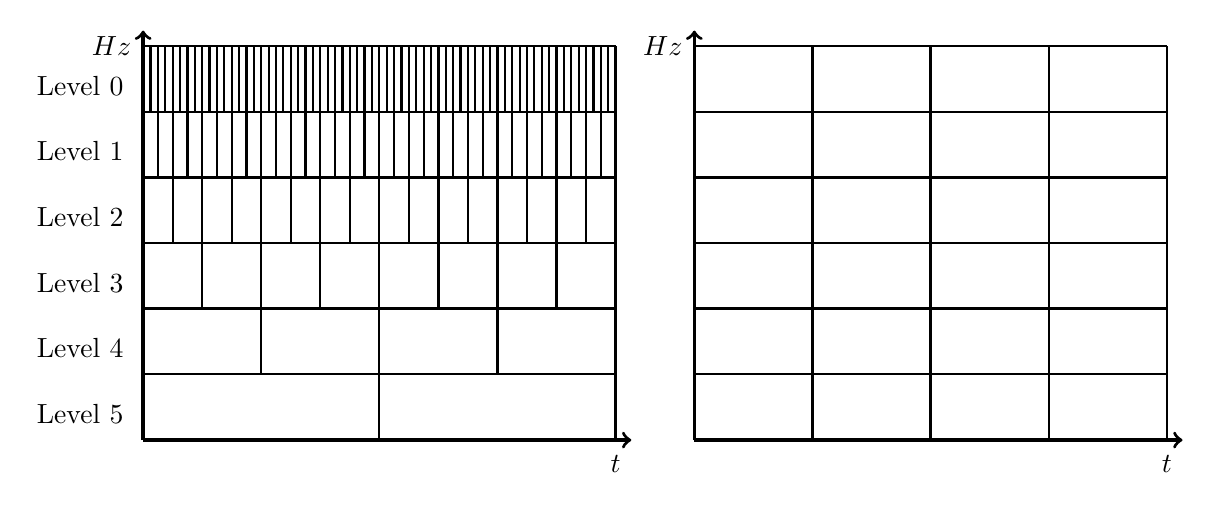
\begin{tikzpicture}
		\draw (6,-5.3) node{$t$};
		\draw (-0.4,0) node{$Hz$};
		
		\draw (-0.8,-0.5) node{Level 0};
		\draw (-0.8,-1.333) node{Level 1};
		\draw (-0.8,-2.166) node{Level 2};
		\draw (-0.8,-2.999) node{Level 3};
		\draw (-0.8,-3.832) node{Level 4};
		\draw (-0.8,-4.665) node{Level 5};
		
		
		\draw[->, very thick] (0,-5)--(0,0.2);
		\draw[->, very thick] (0,-5)--(6.2,-5);
		
		\draw[thick] (0,-0)--(6,-0);
		\draw[thick] (0,-0.833)--(6,-0.833);
		\draw[thick] (0,-1.666)--(6,-1.666);
		\draw[thick] (0,-2.499)--(6,-2.499);
		\draw[thick] (0,-3.33)--(6,-3.33);
		\draw[thick] (0,-4.166)--(6,-4.166);
	
		\draw[thick] (3,-5)--(3,0);
		\draw[thick] (6,-5)--(6,0);
		\draw[thick] (1.5,-4.166)--(1.5,0);
		\draw[thick] (4.5,-4.166)--(4.5,0);
		
		\draw[thick] (0.75,-3.33)--(0.75,0);
		\draw[thick] (2.25,-3.33)--(2.25,0);
		\draw[thick] (3.75,-3.33)--(3.75,0);
		\draw[thick] (5.25,-3.33)--(5.25,0);
		
		\foreach \x in {0,0.375,...,6}
			\draw[thick] (\x,-2.499)--(\x,0);
		
		\foreach \x in {0,0.1875,...,6}
			\draw[thick] (\x,-1.666)--(\x,0);
		
		\foreach \x in {0,0.09375,...,6}
			\draw[thick] (\x,-0.833)--(\x,0);
		
		\draw (13,-5.3) node{$t$};
		\draw (6.6,0) node{$Hz$};
		\draw[->, very thick] (7,-5)--(7,0.2);
		\draw[->, very thick] (7,-5)--(13.2,-5);
		
		\draw[thick] (7,-0)--(13,-0);
		\draw[thick] (7,-0.833)--(13,-0.833);
		\draw[thick] (7,-1.666)--(13,-1.666);
		\draw[thick] (7,-2.499)--(13,-2.499);
		\draw[thick] (7,-3.33)--(13,-3.33);
		\draw[thick] (7,-4.166)--(13,-4.166);
		
		\draw[thick] (8.5,-5)--(8.5,0);
		\draw[thick] (10,-5)--(10,0);
		\draw[thick] (11.5,-5)--(11.5,0);
		\draw[thick] (13,-5)--(13,0);
		\end{tikzpicture}
	}
	\caption{Multiskalenanalyse Auflösung im Vergleich zu STFT Analyse}\label{fig:faauf}
	
\end{figure}

Wie man in der Abbildung \ref{fig:faauf} erkennt übernimmt einem die Multiskalenanalyse das Fenstern. Dabei geht die Wavelet-Transformation einen Kompromiss ein. Im oberen bereich bei den schnelleren Frequenzen sieht man den Zeitpunkt sehr genau. Die tiefen Frequenzen werden dabei wie bei einem Hochpass weggefiltert. In den tieferen Levels sieht man aber trozdem noch die Tiefen Frequenzen. Jedoch sind diese nicht mehr sehr genau auf dem Zeitstrahl abgebildet. Gerade bei der Multiskalenanalyse können durch tiefe Frequenzen an den Rändern oder Sprüngen eines SIgnales Artifkten enstehen.\\





\newpage

